\documentclass[a4paper,10pt]{article}
\usepackage[utf8]{inputenc}
\usepackage{amsmath,mathrsfs}\usepackage{amsmath,amsfonts,amssymb,float,graphicx,mathtools,mathrsfs,tikz,amsthm}


\usepackage{standalone}
\usepackage{caption}
\usepackage{tikz}
\usetikzlibrary{positioning}
\usetikzlibrary{calc}
\usetikzlibrary{backgrounds}
\usepackage{tikzsymbols}
\usepackage{hieroglf}
\usepackage{nameref}
\usepackage{algpseudocode}
\usepackage{hyperref}
\usepackage{natbib}
\usepackage{booktabs}


\definecolor{tip}{rgb}{0.84,0.1,0.11}
\definecolor{branch}{rgb}{.48, .2, .58}
\definecolor{node}{rgb}{.17, .48, .71}
\definecolor{T}{rgb}{.65,.38,.1}

%opening
\title{MTBD models with partner notification}
\author{Anna Zhukova}

\begin{document}

\maketitle

%\begin{abstract}
%
%\end{abstract}

\section{Introduction}
The interaction of epidemiological and evolutionary processes leaves a footprint in pathogen genomes. Phylodynamics leverages this footprint to estimate epidemiological parameters~\cite{Grenfell2004a,Volz2013}. It relies on models that bridge the gap between traditional epidemiology and sequence data by estimating such parameters as the basic reproduction number, $R_0$, from topology and branch lengths of pathogen phylogenies (i.e. genealogies of the pathogen population, approximating the transmission trees) combined with metadata on the samples. This is particularly useful for emerging epidemics, when not enough data (e.g. incidence curves) might be gathered for accurate estimations with classic epidemiological methods, while using genetic data for phylodynamic estimations can provide valuable insights and help prevent epidemic spreads (e.g. accurate estimation of the infectious period is crucial for adjusting health policies for self-isolation).


Phylodynamic models can be classified into two main families:  coalescent~\cite{Volz2009a,Drummond2005,Pybus2000a} and birth-death (BD)~\cite{Kendall1948,Maddison2007,Stadler2009,Stadler2010}. Coalescent models are often preferred for estimating deterministic population dynamics, however for highly stochastic processes, such as the dynamics of emerging pathogens, BD models are better adapted~\cite{Macpherson2021}. In the classic BD model with incomplete sampling (BDS~\cite{Stadler2009}), births represent pathogen transmission events (happening at a constant transmission rate), while deaths correspond to becoming non-infectious (e.g. due to healing, self-isolation, starting a treatment, or death, modelled with a constant removal rate). 

The epidemic spread and detection can however be non-homogenous and depend on different factors, including governmental health policies (e.g. quarantine measures or development of pathogen detection tests), pathogen evolution over time (e.g. some SARS-CoV-2 variants are more transmissible than other),  differences between host individuals (e.g. due to their immune system particularities or to their behaviour).

To allow for heterogeneity at the population level, the multi-type birth-death (MTBD) extention of the classical BDS model was developed by Stadler \textit{et al.}~\cite{Stadler2013a}. MTBD framework allows for different types of individual states (and changes between them, modelled with state change rates). These models are phylodynamic analogies of compartmental models in classical epidemiology (e.g. SIR, Susceptible-Infectious-Removed).  Examples of the MTBD family models include the birth-death exposed-infectious (BDEI) model, which was designed for pathogens featuring an incubation period between the moments of infection and of becoming infectious (e.g. Ebola and SARS-CoV-2), and the birth-death with superspreading model (BDSS) accounting for the fact that some individuals might spread the pathogen more than the others~\cite{Stadler2014}.

To allow for heterogeneity over time, Stadler~\textit{et~al.}~\cite{Stadler2013} developed one-state Bayesian birth-death skyline plot (BDSKY) that divides the time into intervals and allows for different piecewise constant rates on them. K\"{u}hnert \textit{et al.}~\cite{Kuhnert2016} combined the MTBD model with the BDSKY to allow for both piecewise-constant rate changes over time and multiple individual types. In particular the skyline approach can be useful to account for changes in the sampling policies (e.g. before/after HIV discovery or before/after PCR test spread for SARS-CoV-2).


Another important source of heterogeneity that none of these models account for is inflicted by non-random sampling. We can propose different sampling probabilities for different types of individuals in MTBD framework, or change of the sampling probability over time intervals with the BDSKY, however, none of them can account for non-randomness of sampling, in particular due to contact tracing and partner notification. 

In this study we propose an extension of the MTBD framework that allows to model non-random sampling due to partner notification, MTBD-PN. In the rest of the article, we describe the MTBD-PN model family and its assumptions, implement a transmission tree simulator under these models, derive the equations for their likelihood calculation, implement a maximum likelihood parameter estimator and test it on simulated data. We also propose a test allowing to distinguish between MTBD and MTBD-PN models. Finally, we apply it to the study of HIV epidemic in the UK.


\section{MTBD-PN Framework}
In a pathogen transmission tree $\mathscr{T}$ (approximated by a time-scaled pathogen phylogeny) the tips represent sampled pathogens, patient state transitions occur along the branches, and bifurcations (i.e. internal nodes) correspond to pathogen transmissions (Fig.~\ref{fig:tt}). The tree branches are measured in units of time, where $T$ is the time that passed between the tree root (the beginning of the (sub-)epidemic) and the last sampled tip. 


\begin{figure*}[tbhp]
\centering 
%\includegraphics[width=0.8\textwidth]{Transmission_tree.png}
\includestandalone[width=1\textwidth]{Fig_tree}
\caption{A transmission tree $\mathscr{T}$ with $n=5$ external nodes (i.e. tips, which correspond to sampling events: $0000, 0001, 001, 010, 011$), $n-1=4$ internal nodes (which correspond to transmissions: $0$ (the root) and $00, 01, 000$) and $2n - 2 = 8$ branches (plus the root branch of zero length). %The lengths of the branches are shown on the right of each branch: $t_i$ is the lengths of the branch connecting the node $i$ to its parent. 
Time $t$ starts at the root of the tree ($t=0$) and goes till the last sampled tip. The times of the nodes are shown on the left, e.g. $t_{0001}$ is the time of tip $0001$ (when $0001$'s pathogen was sampled). $T$ corresponds to the end of the sampling period (when the most recent tip, $0000$, was sampled).}
\label{fig:tt} 
\end{figure*}

\subsection{MTBD Framework}
A general MTBD model describes $m$ possible individual states. An individual in state $k \in 1:m$ can be removed (i.e., become non-infectious, e.g., due to healing, starting a treatment, self-isolation, or death) at a rate $\psi_k$, change their state to a state $l \in 1:m$ at a rate $\mu_{kl}$ (where $\mu_{kk} = 0$), and transmit their pathogen to an individual in a state $l \in 1:m$ at rate $\lambda_{kl}$. Upon $i$'s removal, their pathogen can be sampled (and hence observed as a tip in the transmission tree) with a probability $\rho$. 

The MTBD model can be described with master equations representing the likelihood densities of evolving as on the observed transmission tree, with time $t$ going forward from the root ($t=0$) till the time of the last sampled tip ($t=T$). These likelihood densities depend on the probability $U_s(t)$ of an unobserved transmission tree that started from one individual at time $t$ in state $s \in 1:m$ and evolved till $T$, without them or any of their induced cases being sampled: 

\begin{equation}
\scriptsize
\begin{cases}
\dot{U}_{s}(t) = &\Big(\sum\limits_{k=1}^{m} \mu_{sk} + \sum\limits_{k=1}^{m} \lambda_{sk} + \psi_s\Big) U_{s}(t)\; \textit{\color{gray} $\leftarrow$ no event in the next infinitesimal time $\Delta t$ }\\ 
    & - \sum\limits_{k=1}^{m} \mu_{sk} U_{k}(t)\;  \textit{\color{gray} $\leftarrow$ change of the state, folowed by unsampled evolution from the new state }\\
    &- \sum\limits_{k=1}^{m} \lambda_{sk} U_{s}(t)U_{k}(t) \;  \textit{\color{gray} $\leftarrow$ transmission, followed by unsampled evolutions of both subtrees}\\
    &- \psi_s (1 - \rho)\;  \textit{\color{gray} $\leftarrow$ removal without sampling}\\
U_{s}(T) = & 1\;  \textit{\color{gray} $\leftarrow$ the probability to stay unsampled over time 0 is 1} \label{eq:u}
\end{cases}
\end{equation}


With the equations~(\ref{eq:u}), we can write down the equations for the probability densities $p_{s,si}^{(i)}(t)$ of evolving as on an observed tree branch that finishes at time $t_i$ in state $si$, starting  on this branch at a time $t \leq t_i$ in state $s$. The master equations for the MTBD models were initially developed by ~\citet{Stadler2013a}, however here we present their parallelizable version that we recently proposed~\cite{zhukovaFastAccurateMaximumLikelihood2022}:

\begin{equation}
\scriptsize
\begin{cases}
\dot{p}_{s,si}^{(i)}(t) = & \Big(\sum\limits_{k=1}^{m} \mu_{sk} + \sum\limits_{k=1}^{m} \lambda_{sk} + \psi_s\Big) p_{s,si}^{(i)}(t)\; \textit{\color{gray} $\leftarrow$ no event in the next infinitesimal time $\Delta t$ }\\
    & - \sum\limits_{k=1}^{m} \mu_{sk} p_{k,si}^{(i)}(t)\;  \textit{\color{gray} $\leftarrow$ change of the state, folowed by evolution from the new state }\\
    & - \sum\limits_{k=1}^{m} \lambda_{sk} p_{s,si}^{(i)}(t)U_{k}(t)\;  \textit{\color{gray} $\leftarrow$ transmission, where the recipient subtree stayed unsampled}\\
    & - \sum\limits_{k=1}^{m} \lambda_{sk} p_{k,si}^{(i)}(t)U_{s}(t)\;  \textbf{\textit{\color{gray} $\leftarrow$ transmission, where the donor subtree stayed unsampled}}\\
p_{s,si}^{(i)}(t_i) = & 
    \begin{cases}
    0 & \textit{\color{gray} if $i$ is in state $k \neq si$}\\
    1 & \textit{\color{gray} if $i$ is in state $si$}
    \end{cases}\label{eq:p}
\end{cases}
\end{equation}

If the states of all the observed tree $\mathscr{T}$ nodes are known, then its likelihood density under parameter values $\Theta$ can be calculated as $L(\mathscr{T}|\Theta)$:

{\scriptsize
\begin{alignat*}{3}
log L(\mathscr{T}|\Theta) =  \sum\limits_{i \in tips}  log(&\psi_{si}  \rho) & \textit{\color{gray} $\leftarrow$ sampling of $n$ tips} \\
 +\sum\limits_{i \in \textit{internal nodes}} log \Big(&\sum\limits_{k=1}^{m} \lambda_{si,k}  & \textit{\color{gray} $\leftarrow$ $n - 1$ transmission events}\\
 & \cdot \big(p_{si,si0}^{(i0)}(t_i)p_{k,si1}^{(i1)}(t_i) + p_{k,si0}^{(i0)}(t_i)p_{si,si1}^{(i1)}(t_i)\big)\Big) & \textit{\color{gray}$\leftarrow$ child branch evolutions}  \label{eq:mtbd_tree_likelihood}
\end{alignat*}}


\subsection{PN extension}

We now propose a non-Markovian extension of the MTBD framework that adds partner notification (PN), for a tree with known node states.  In MTBD-PN, at the moment of sampling the sampled individual might notify their most recent partner with a given probability $\rho_n$. Upon notification, partner is removed almost instantaneously (modelled via a notified removal rate $\psi_n >> \psi_k \;\forall k \in 1:m$). MTBD-PN hence has $2k^2 + 1$ classical MTBD and 2 additional parameters:
\begin{itemize}
 \item $\mu_{kl} \;\forall k,l \in 1:m, k \neq l$ -- state change rate from $k$ to $l$;
 \item $\lambda_{kl} \;\forall k,l \in 1:m$ -- transmission rate: an infected individual in state $k$ transmits their pathogen (which corresponds to an internal node in the transmission tree), the newly infected individual is in state $l$;
 \item $\psi_k \;\forall k \in 1:m$ -- removal rate: an infected individual in state $k$ stops being infectious at this rate (exponential distribution), which corresponds to a tip in the transmission tree (observed or hidden);
 \item $\rho$ -- sampling probability: upon removal the individual's pathogen might get sampled with this probability, which corresponds to an observed tip in the transmission tree;
 \item $\rho_n$ -- notification probability: upon sampling, the sampled individual might notify their most recent partner with this probability;
 \item $\psi_n >> \psi_k  \;\forall k \in 1:m$ -- notified removal rate: a notified individual stops being infectious and gets observed with this rate (exponential distribution), which corresponds to an observed tip in the transmission tree.
\end{itemize}


This model is a simplification of the notification process, in particular it makes 5 assumptions, which might need to be relaxed in the future work:
\begin{enumerate}
\item only observed individuals can notify (instead of any removed individual);
\item notified individuals are always observed upon removal;
\item notified individuals do not notify further;
\item after the notification notified individuals do not transmit further;
\item only the most recent partner can get notified.
\end{enumerate}

These assumptions make the mathematics behind the model manageable, however they can be easily relaxed in a simulator (e.g. to be used with a deep learning estimator~\cite{Voznica2021} after).

\subsection{Mathematical formulation}
$p_{s,si}^{(i)}(t)$ in equations~(\ref{eq:p}) describes an evolution along a tree branch, provided that we do not know whether the individual at the end of the branch (at time $t_i$) is the same as at time $t$. They could be different if a hidden transmission, where the donor subtree stayed unobserved, occurred between times $t$ and $t_i$.

We will use an \textbf{oriented probability} $P^{(i,o)}_{s,si}(t)$ for the cases when the individual at the end of the branch is the same as at time $t$:

\begin{equation}
\scriptsize
\begin{cases}
\dot{p}_{s,si}^{(i,o)}(t) = & \Big(\sum\limits_{k=1}^{m} \mu_{sk} + \sum\limits_{k=1}^{m} \lambda_{sk} + \psi_s\Big) p_{s,si}^{(i,o)}(t)\; \textit{\color{gray} $\leftarrow$ no event in the next infinitesimal time $\Delta t$ }\\
    & - \sum\limits_{k=1}^{m} \mu_{sk} p_{k,si}^{(i,o)}(t)\;  \textit{\color{gray} $\leftarrow$ change of the state, folowed by evolution from the new state }\\
    & - \sum\limits_{k=1}^{m} \lambda_{sk} p_{s,si}^{(i,o)}(t)U_{k}(t)\;  \textit{\color{gray} $\leftarrow$ transmission, where the recipient subtree stayed unsampled}\\
p_{s,si}^{(i,o)}(t_i) = & 
    \begin{cases}
    0 & \textit{\color{gray} if $i$ is in state $k \neq si$}\\
    1 & \textit{\color{gray} if $i$ is in state $si$}
    \end{cases}\label{eq:p-o}
\end{cases}
\end{equation}


Additionally we define a \textbf{non-hidden probability} $p^{(i,nh)}_{s,si}(t)$ for the cases when no hidden transmission occurred along the branch:

\begin{equation}
\scriptsize
\begin{cases}
\dot{p}_{s,si}^{(i,nh)}(t) = & \Big(\sum\limits_{k=1}^{m} \mu_{sk} + \sum\limits_{k=1}^{m} \lambda_{sk} + \psi_s\Big) p_{s,si}^{(i,nh)}(t)\; \textit{\color{gray} $\leftarrow$ no event in the next infinitesimal time $\Delta t$ }\\
    & - \sum\limits_{k=1}^{m} \mu_{sk} p_{k,si}^{(i,nh)}(t)\;  \textit{\color{gray} $\leftarrow$ change of the state, folowed by evolution from the new state }\\
p_{s,si}^{(i,nh)}(t_i) = & 
    \begin{cases}
    0 & \textit{\color{gray} if $i$ is in state $k \neq si$}\\
    1 & \textit{\color{gray} if $i$ is in state $si$}
    \end{cases}\label{eq:p-nh}
\end{cases}
\end{equation}

Under the MTBD-PN model, the probability density $q_{si,sj}(i)$ of a branch connecting a node $i$ in state $si$ to its parent node $j$ in state $sj$ can be written as:


\begin{equation}
\scriptsize
q_{sj,si}(i) = 
\begin{cases}
q^{(u)}_{sj,si}(i) = p^{(i)}_{sj,si}(t_j) \textit{\color{gray} ~~if $i$ is an \textbf{unnotified non-notifier}}\\
q_{sj,si}^{(n)}(i) = 
p_{sj,si}^{(i,nh)}(t_j) \textit{\color{gray} ~~if $i$ is a tip corresponding to a \textbf{notifier}}\\
~~~~~~~~~~~~ \textit{\color{gray}(parent is the last transmission, no hidden transmission along the branch)}
\\
q^{(p)}_{sj,si}(i)  = p^{(i, o)}_{sj,si}(t_j)  \textit{\color{gray} ~~if $i$ is an internal node who will be notified after $t_i$}
\\
q^{(p)}_{sj,si}(i, r)  = p^{(r, o)}_{sj,si}(t_j) e^{- \psi_n (t_i - t_r)} \textit{\color{gray} if $i$ is a \textbf{partner} tip notified by $r$ at time $t_r < t_i$}\\
\end{cases}
\label{eq:branch}
\end{equation}

Using the formulas~(\ref{eq:branch}), we can calculate the likelihood density of a tree using a pruning algorithm~\cite{10.1093/sysbio/22.3.240}, where for each visited node $i$ we calculate two values for each possible state $sj \in 1:m$ at the beginning of the branch connecting it to its parent $j$: the likelihood density of its subtree if its branch corresponds to (1) an unnotified individual $l^{(u)}_{sj}(i)$; (2) a notifier $l^{(u)}_{sj}(i)$ (for tips only); or (3) an (eventually) notified partner $l^{(p)}_{sj}(i, r)$ (notified by $r$).

For a tip $i$, these values can be calculated by considering all its possible states $si \in 1:m$, as:
\begin{equation}
\scriptsize
\begin{array}{ll}
l^{(u)}_{sj}(i) &= \sum\limits_{si=1}^{m} q^{(u)}_{sj,si}(i)\psi_{si}\rho (1-\rho_{n})\\
l^{(n)}_{sj}(i) &= \sum\limits_{si=1}^{m} q^{(n)}_{sj,si}(i)\psi_{si}\rho \rho_{n}\\
l^{(p)}_{sj}(i, r) &= \sum\limits_{si=1}^{m} q^{(p)}_{sj,si}(i,r)\psi_{n}\\
\end{array}
\label{eq:tip}
\end{equation}

Let us now consider an internal node $i$ in state $si$ with two child nodes, $i0$ and $i1$. We will start with the configuration where the $i$'s branch corresponds to an unnotified individual:

\begin{equation}
\scriptsize
\begin{split}
l^{(u)}_{sj}(i) = &\sum\limits_{si=1}^{m}q^{(u)}_{sj,si}(i) \sum\limits_{k=1}^{m} \lambda_{si,k} \\
\cdot \Big(~&
l^{(u)}_{si}(i0)l^{(u)}_{k}(i1) + l^{(u)}_{k}(i0)l^{(u)}_{si}(i1)  \textit{\color{gray} $\leftarrow$ no notification on child branches} \\
& + is\_tip(i0) \big(l^{(n)}_{si}(i0)l^{(p)}_{k}(i1,i0) + l^{(n)}_{k}(i0)l^{(p)}_{si}(i1,i0) \big)\textit{\color{gray} $\leftarrow$ notification of someone in $i1$'s subtree by $i0$} \\
&+ is\_tip(i1) \big(l^{(p)}_{si}(i0,i1)l^{(n)}_{k}(i1) + l^{(p)}_{k}(i0,i1)l^{(n)}_{si}(i1) \big)~\Big) \textit{\color{gray} $\leftarrow$ notification of someone in $i0$'s subtree by $i1$},\\
\textit{where } & is\_tip(r) = 1 \textit{ if r is a tip and $= 0$ if r is an internal node.}
\end{split}\label{eq:lu}
\end{equation}

Note that a notification will only be possible if (1) the notifying branch is external (as the notifier only notifies the most recent partner); (2) there is at least one tip in the notified subtree that can be a partner, i.e. was sampled after the notifier and whose parent's time was before notification (i.e. there was no transmission between notification and sampling). 

In the other case (when an internal nodes's branch corresponds to a partner who will eventually get notified by a node $r$), the individual on the path connecting this branch to the notified tip stays the same (the partner). Hence, all the transmissions on this path are oriented and correspond to the partner transmitting to another recipient individual. Moreover, this recipient's branch cannot be notified by our partner (as in our model notified partners do not notify further):

 
\begin{equation}
\scriptsize
\begin{split}
l^{(p)}_{sj}(i, r) = \sum\limits_{si=1}^{m}q^{(p)}_{sj,si}(i,r) \sum\limits_{k=1}^{m}  \lambda_{si,k}\Big(&l^{(p)}_{si}(i0,r)l^{(u)}_{k}(i1) \textit{\color{gray} $\leftarrow$ notification in $i0$'s subtree} \\
 &+ l^{(u)}_{k}(i0)l^{(p)}_{si}(i1,r)\Big)  \textit{\color{gray} $\leftarrow$ notification in $i1$'s subtree} 
\end{split}\label{eq:lu}
\end{equation}

Note that $l^{(p)}_{sj}(i, r)$ depends on the notifier $r$ and can only be calculated once the notification time is known, i.e. once we have climbed to an internal node corresponding to the transmission between the notifier (corresponding to one of its children, must be a tip) and the partner (the other child). As only the contributions coming from the partner tip branches depend on the notification times, while climbing the tree for each internal node $i$ and each of the possible states $sj \in 1:m$ at the beginning of its branch, we can store an array of pre-calculated values for notified internal paths for each of its tips (e.g. $a$) and each of the states $v \in 1:m$ at the beginning of $a$'s branch, describing the tip's sampling time $t_a$ and a configuration $C_{sj}(i,a,v)$: 

\begin{equation}
\scriptsize
\begin{split}
C_{sj}(i,a,v) = &\begin{cases}
q^{(p)}_{sj,v}(i)
\sum\limits_{k=1}^{m}\lambda{v,k} \cdot l_{k}^{(u)}\Big(child(i, \not a)\Big) \textit{\color{gray}~~~if $i$ is a direct parent of $a$}
\\
\sum\limits_{si=1}^{m}q^{(p)}_{sj,si}(i)
\sum\limits_{k=1}^{m}\lambda{si,k} \cdot l_{k}^{(u)}\Big(child(i, \not a)\Big)C_{si}\Big(child(i, a),a,v\Big) \textit{\color{gray}~~otherwise}\\ 
\end{cases},
\\ &\textit{where child(i,a) is the child of i whose subtree contains a},
\\
 &\textit{~~~~~~~~child(i,$\not a$) is the child of i whose subtree does not contain a.}
\end{split}
\label{eq:c}
\end{equation}

%Note that the path connecting $j$ to the parent of $i$ in this configuration corresponds to the same partner individual, hence this individual is the donor at all transmissions (internal nodes) on this path, hence at the moments of these transmissions the individual's state is known (as we only consider trees with known node states). At each internal node in this path the other branch (leading to a non-$j$'s subtree) corresponds to a recipient of the transmission occurring at that node, where the donor is the partner individual corresponding to $j$ (and $i$) and hence will not notify the recipient (as in our model's assumptions notified partners do not notify further).

Once a potential notifier tip $r$ is identified (i.e., $r$ is a sister tip of the currently visited node $i$), we can calculate $l^{(p)}_{sj}(i, r)$ as:
\begin{equation}
\scriptsize 
l^{(p)}_{sj}(i, r) = \sum\limits_{a \in tips(i)}\sum\limits_{k=1}^{m} C_{sj}(i, a, k) l^{(p)}_{k}(a, r)\label{eq:lp}
\end{equation}


Finally, the tree $\mathscr{T}$ likelihood density $\mathscr{L}(\mathscr{T}|\Theta)$ under MTBD-PN model with parameters $\Theta$ can be calculated as $l^{(u)}_{state(root)}(root)$, as the root can only correspond to an unnotified individual (since there was no observed transmission before it).

%The computational of $\mathscr{L}(\mathscr{T}|\Theta)$ includes $O(N^2)$ resolutions of system~(\ref{eq:p}) (for different times and initial conditions) in the worst case (caterpillar tree) and $O(NlogN)$ in the best case (for a balanced tree), where $N$ is the number of tips in $\mathscr{T}$.

\subsection{BD-PN}
A particular example of the MTBD model generating trees with known node states is the basic birth-death model~\citep{Stadler2009} where all the individuals are in the same state. They can transmit with a constant rate $\lambda$, get removed with a constant rate $\psi$, be sampled upon removal with a probability $\rho$. Below we describe the special case of equations~(\ref{eq:u}-\ref{eq:lp}) for its PN extension BD-PN.

The master equation for this model are a simplified version of the general case:

\begin{equation}
\scriptsize
\begin{cases}
\dot{U}(t) &= \Big(\lambda + \psi\Big) U(t) - \lambda U^2(t) - \psi (1 - \rho)\\\\
U(T) &=  1\\
\dot{p}^{(i)}(t) &=  \Big(\lambda + \psi\Big) p^{(i)}(t) - 2 \lambda p^{(i)}(t)U(t)\\
\dot{p}^{(i,o)}(t) &=  \Big(\lambda + \psi\Big) p^{(i)}(t) - \lambda p^{(i)}(t)U(t)\\
\dot{p}^{(i,nh)}(t) &=  \Big(\lambda + \psi\Big) p^{(i)}(t)\\
p^{(i)}(t_i) &= p^{(i,o)}(t_i) = p^{(i,nh)}(t_i) = 1
\end{cases}
\end{equation}


These equations have the following closed form solutions:
\begin{equation}
\scriptsize
\begin{split}
&\begin{cases}
U(t) = \frac{\lambda + \psi + c_1 \frac{c_2 e^{t c_1} - 1}{c_2 e^{tc_1} + 1}}{2\lambda}\\
\\
p^{(i)}(t) = \frac{c_3^2 e^{c_1 (t - t_i)}}{(c_2e^{c_1 t} + 1)^2} \\
\\
p^{(i,o)}(t) =  \frac{c_3 e^{1/2 (\lambda + \psi + c_1)(t - t_i)}}{c_2e^{c_1 t} + 1} \\
\\
p^{(i,nh)}(t) =  e^{(\lambda + \psi)(t - t_i)}
\end{cases},\\
& \textit{where } c_1 = \sqrt{(\lambda - \psi)^2 + 4 \lambda\psi\rho},\; c_2 = \frac{c_1 + \lambda - \psi}{c_1 - \lambda + \psi}e^{-Tc_1},\; c_3 = c_2 e^{c_1 t_i} + 1
\end{split}
\end{equation}


The likelihood of a tree $\mathscr{T}$ under BD-PN model with parameter values $\Theta$ can be calculated as $\mathscr{L}(\mathscr{T}|\Theta) = l^{(u)}(root)$, where $l^{(u)}(i)$ is a likelihood of node $i$'s subtree if the branch connecting $i$ to its parent node (of length zero for the root) correspond to an unnotified individual. It can be calculated, along with $l^{(p)}(i, r)$ (likelihood when $i$'s branch corresponds to an eventually notified partner, notified by $r$) for each tree node $i$ with a pruning algorithm.


For a tip $i$ whose branch starts at time $t_j$ and finishes at time $t_i$, these values can be calculated as:
\begin{equation}
\scriptsize
\begin{array}{ll}
l^{(u)}(i) &= p^{(i)}(t_j)\psi\rho (1-\rho_{n})\\
l^{(n)}(i) &= p^{(i,nh)}(t_j)\psi\rho \rho_{n}\\
l^{(p)}(i, r) &= p^{(r,o)}(t_j)e^{-\psi_n (t_i - t_r)}\psi_{n}\\
\end{array}
\end{equation}

For an internal node $i$ whose branch starts at time $t_j$ and finishes at time $t_i$, with two child nodes, $i0$ and $i1$, these values can be calculated as:

\begin{equation}
\scriptsize
\begin{array}{ll}
l^{(u)}(i) &= p^{(i)}(t_j) 2\lambda 
\Big(l^{(u)}(i0)l^{(u)}(i1) 
+ is\_tip(i0) l^{(n)}(i0)l^{(p)}(i1,i0)
+ is\_tip(i1) l^{(p)}(i0,i1)l^{(n)}(i1)\Big),\\
& \textit{where } is\_tip(x) = 1 \textit{ if x is a tip and $= 0$ if x is an internal node.}\\
l^{(p)}(i, r) &= p^{(i,o)}(t_j) \lambda\Big(l^{(p)}(i0,r)l^{(u)}(i1) + l^{(u)}(i0)l^{(p)}(i1,r)\Big),\\
& \textit{where r is the notifier.}\\
\end{array}
\end{equation}

As in the general MTBD-PN case, $l^{(p)}(i, r)$ depends on the notifier $r$ and can only be calculated once the notification time is known, i.e. once we have climbed to an internal node corresponding to the transmission between the notifier (corresponding to one of its children, must be a tip) and the partner (the other child). As only the contributions coming from the partner tip branches depend on the notification times, while climbing the tree for each internal node $i$ and the time of its branch start $t_j$, we can store an array of pre-calculated values for notified internal paths for each of its tips (e.g. $a$), describing the tip's sampling time $t_a$ and a configuration $C(i,a)$: 

\begin{equation}
\scriptsize
\begin{split}
C(i,a) = &\begin{cases}
1 \textit{\color{gray}~~~if $i == a$}
\\
p^{(i,o)}(t_j) \lambda \cdot l^{(u)}\Big(child(i, \not a)\Big)C\Big(child(i, a),a\Big) \textit{\color{gray}~~otherwise}\\ 
\end{cases},
\\ &\textit{where child(i,a) is the child of i whose subtree contains a},
\\
 &\textit{~~~~~~~~child(i,$\not a$) is the child of i whose subtree does not contain a.}
\end{split}
\end{equation}

Once a potential notifier tip $r$ is identified (i.e., $r$ is a sister tip of the currently visited node $i$), we can calculate $l^{(p)}(i, r)$ as:
\begin{equation}
\scriptsize 
l^{(p)}(i, r) = \sum\limits_{a \in tips(i)}C(i, a) l^{(p)}(a, r)
\end{equation}




\subsection{BDEI-PN}
Another particular example of the MTBD model generating trees with known node states is the basic birth-death exposed-infectious model (BDEI)~\citep{Stadler2014} where   infectious ($I$) individuals can transmit (at a rate $\lambda$) or be removed (at a rate $\psi$), and hence create an internal or external node in the transmission tree. Upon removal they can be sampled with a probability $\rho$. The recipient of the transmission is at first in state $E$ (exposed, already infected but not yet infectious), they can eventually become infectious ($I$) at a state-change rate $\mu$. No other type of state transitions, transmissions or removals are allowed. Below we describe the special case of equations~(\ref{eq:u}-\ref{eq:lp}) for its PN extension BDEI-PN, assuming only infectious individuals can be removed and sampled even with notification (e.g., because the viral load of the exposed individuals is yet undetectable).


The master equations for the BDEI-PN model are a special case of the MTBD-PN equations:

\begin{equation}
\scriptsize
\begin{cases}
\dot{U_E}(t) = &\mu U_E(t)- \mu U_I(t)\\    
\dot{U_I}(t) = &\Big(\lambda + \psi\Big) U_I(t)- \lambda U_I(t)U_E(t)- \psi (1 - \rho)\\
U_E(T) = & U_I(T) = 1\\
\dot{p}_E^{(i)}(t) = & \mu p_E^{(i)}(t) - \mu p_I^{(i)}(t)\\
p_E^{(i)}(t_i) = & 0\\
p_E^{(i,o)}(t_i) = & p_E^{(i,nh)}(t_i) = p_E^{(i)}(t_i)\\
\dot{p}_I^{(i)}(t) = & \Big(\lambda + \psi\Big) p^{(i)}(t) - \lambda \Big(p_I^{(i)}(t)U_E(t) + p_E^{(i)}(t)U_I(t)\Big)\\
\dot{p}_I^{(i,o)}(t) = & \Big(\lambda + \psi\Big) p^{(i,o)}(t) - \lambda p_I^{(i,o)}(t)U_E(t)\\
\dot{p}_I^{(i,nh)}(t) = & \Big(\lambda + \psi\Big) p^{(i,nh)}(t)\\
p_I^{(i)}(t_i) = & p_I^{(i,o)}(t_i) = p^{(i,nh)}(t_i) = 1\label{eq:up-bd}
\end{cases}
\end{equation}

The likelihood of a tree $\mathscr{T}$ under BDEI-PN model with parameter values $\Theta$ can be calculated as $\mathscr{L}(\mathscr{T}|\Theta) = l_I^{(u)}(root)$, where $l_s^{(u)}(i)$ is a likelihood of node $i$'s subtree if the branch connecting $i$ to its parent node (of length zero for the root) starts in state $s \in \{E, I\}$ and correspond to an unnotified individual. It can be calculated, along with $l_s^{(p)}(i, notifier)$ (likelihood when $i$'s branch corresponds to an eventually notified partner) for each tree node $i$ with a pruning algorithm.


For a tip $i$ whose branch starts at time $t_j$ in state $s \in \{E, I\}$ and finishes at time $t_i$ in state $I$, these values can be calculated as:
\begin{equation}
\scriptsize
\begin{array}{ll}
l^{(u)}_{s}(i) &= p_s^{(i)}(t_j)\psi\rho (1-\rho_{n})\\
l^{(n)}_{s}(i) &= p_s^{(i,nh)}(t_j)\psi\rho \rho_{n}\\
l^{(p)}_{s}(i, r) &= p_s^{(r,o)}(t_j)e^{-\psi_n (t_i - t_r)}\psi_{n}\\
\end{array}
\end{equation}

For an internal node $i$ whose branch starts at time $t_j$ is state $s$ and finishes at time $t_i$ in state $I$, with two child nodes, $i0$ and $i1$, these values can be calculated as:

\begin{equation}
\scriptsize
\begin{array}{ll}
l^{(u)}(i) =& p_s^{(i)}(t_j) \lambda \\
& \cdot \Big(\big(l_I^{(u)}(i0)l_E^{(u)}(i1) + l_E^{(u)}(i0)l_I^{(u)}(i1)\big) \\
&~~+ is\_tip(i0) \big(l_I^{(n)}(i0)l_E^{(p)}(i1,i0) + l_E^{(n)}(i0)l_I^{(p)}(i1,i0)\big)\\
&~~+ is\_tip(i1) \big(l_I^{(p)}(i0,i1)l_E^{(n)}(i1) + l_E^{(p)}(i0,i1)l_I^{(n)}(i1)\big)\Big),\\
& \textit{where } is\_tip(x) = 1 \textit{ if x is a tip and $= 0$ if x is an internal node.}\\
l^{(p)}(i, r) &= p_s^{(i,o)}(t_j) \lambda\Big(l_I^{(p)}(i0,r)l_E^{(u)}(i1) + l_E^{(u)}(i0)l_I^{(p)}(i1,r)\Big),\\
& \textit{where r is the notifier.}\\
\end{array}
\end{equation}

As in the general MTBD-PN case, $l_s^{(p)}(i, r)$ depends on the notifier $r$ and can only be calculated once the notification time is known, i.e. once we have climbed to an internal node corresponding to the transmission between the notifier (corresponding to one of its children, must be a tip) and the partner (the other child). As only the contributions coming from the partner tip branches depend on the notification times, while climbing the tree for each internal node $i$ and each state $s \in \{E, I\}$ at the time of its branch start $t_j$, we can store an array of pre-calculated values for notified internal paths for each of its tips (e.g. $a$), describing the tip's sampling time $t_a$ and a configuration $C_s(i,a)$. Note, that the partner branch for any transmission after the transmission between the notifier and the partner, is always the donor one (hence, starting in state $I$).

\begin{equation}
\scriptsize
\begin{split}
C_s(i,a) = &\begin{cases}
1 \textit{\color{gray}~~~if $i==a$}
\\
p_s^{(i,o)}(t_j) \lambda \cdot l_E^{(u)}\Big(child(i, \not a)\Big)C_I\Big(child(i, a),a\Big) \textit{\color{gray}~~otherwise}\\ 
\end{cases},
\\ &\textit{where child(i,a) is the child of i whose subtree contains a},
\\
 &\textit{~~~~~~~~child(i,$\not a$) is the child of i whose subtree does not contain a.}
\end{split}
\end{equation}

Once a potential notifier tip $r$ is identified (i.e., $r$ is a sister tip of the currently visited node $i$), we can calculate $l_s^{(p)}(i, r)$ as:
\begin{equation}
\scriptsize 
l_s^{(p)}(i, r) = 
\begin{cases}
\sum\limits_{a \in tips(i)}C_s(i, a) l_I^{(p)}(a, r)\textit{\color{gray}~~if $i$ is an internal node or $s=I$}\\
l_E^{(p)}(a, r)\textit{\color{gray}~~if $i=a$ and $s=E$}
\end{cases}
\end{equation}

\subsection{Extension to forests}

As we previously described in~\citep{zhukovaFastAccurateMaximumLikelihood2022}, the likelihood calculation with MTBD models can be easily extended to forests. This extension applies also to MTBD-PN models. Forests are useful for cases when a (sub-)epidemic started with several infected individuals (e.g. dur to multiple pathogen introductions to a country of interest or due to a change of health policies leading to a change in parameter values).

In this case the (sub-)epidemic leads to a forest $\mathscr{F}$ of $f$ observed trees: $\mathscr{T}_1, \ldots, \mathscr{T}_f$. If all the trees started at the same time (e.g. due to health policy change), the forest might also include a certain number $u$ of unobserved trees, i.e., individuals who were infected at the beginning of the (sub-)epidemic, but whose trees stayed unobserved  as none of their tips got sampled.
Forest likelihood formula hence combines the likelihoods of $f$ observed and $u$ hidden trees, and can be represented in logarithmic form~(\ref{eq:forest_likelihood}). Tree likelihood formula %[\ref{eq:tree_likelihood}] 
is its special case, where $f=1$ and $u=0$. 

%As our application to Ebola data (see~Application) shows, $u$ is an important parameter: while the results are not very sensible to slight $u$ variations, ignoring it completely (e.g. using $u=0$ instead of $u \approx 500$ in our example) can change the inferences.

\begin{equation}
logL(\mathscr{F}|\Theta,u)=u\,logU_{hidden}(\Theta) + \sum\limits_{j=1}^f logL(\mathscr{T}_j|\Theta), \textit{ where } U_{hidden}(\Theta)=\sum\limits_{s=1}^{d}\pi_s U_s(0) \label{eq:forest_likelihood} 
\end{equation}

If all the sub-epidemics started at the same time, for given model parameter values $\Theta$ we can estimate the number of hidden trees $u$ from the number of observed trees $f$ as:
\begin{equation}
u = f \frac{U_{hidden}(\Theta)}{1 - U_{hidden}(\Theta)}\label{eq:u} 
\end{equation}



\section{Tree simulator}
We implemented a quick tree simulator that generates sampled transmission trees under MTBD and MTBD-PN models (with $m$ states). The simulator is Gillespie-based, generates state change, transmission and removal times, and only reconstructs the sampled parts of the tree to save memory and increase speed. 

The simulator iterates through occurring events till either time or sampled tip number limit is reached. 
It keeps updating an array $C = [c_1, \ldots, c_m]$ of counts of currently infected individuals (i.e. non-removed) in different states; an array $S = [s_1, \ldots, s_m]$ of counts of sampled individuals in different states; as well as a mapping $M$ between states and ids of currently infected individuals in those states, and a mapping $N$ between states and ids of sampled individuals in those states.  In the beginning ($t=0$) the only infected individual corresponds to the root: $c_k = 0, \;M_k = \emptyset \; \forall k \in 1:m, \; k \neq state(root)$, $c_{state(root)} = 1, \; M_{state(root)} = \{root\}$, and no individual is sampled: $s_k=0,\;N_k = \emptyset \; \forall k \in 1:m$.

At each iteration the algorithm (1) calculates the time of the next event; (2) chooses the type of this event and the the individual involved in it; (3) updates the counts and the mappings according to the event and records its time.

At step 1, to calculate the time of the next event, we (i) calculate the total rate $r$ as a sum of total state change, transmission and transition rates: $r = r^{(\mu)} + r^{(\lambda)} + r^{(\psi)}$, where $r^{(\mu)} = \sum\limits_{k=1}^{m} c_k \sum\limits_{r=1}^{m} \mu_{kr}$, $r^{(\lambda)} = \sum\limits_{k=1}^{m} c_k \sum\limits_{r=1}^{m} \lambda_{kr}$, and $r^{(\psi)} = \sum\limits_{k=1}^{m} c_k \psi_{k}$; (ii) draw $\Delta t$ from the exponential distribution with rate $r$; (iii) update the current time to $t + \Delta t$.

At step 2, to chose the type of the event, we draw a value $v$ (uniformly) from an interval $[0, r[$. This interval can be seen as composed of subintervals corresponding to each possible event, where the width of each subinterval is defined by the corresponding rate and infected individual count, e.g. the subinterval corresponding to a transmission from $k$ to $r$ has a width of $\lambda_{kr}c_k$. The subinterval in which $v$ is located defines the event type.

At step 3, we randomly draw an individual $i$ of type $k$ (selected at step 2) from $M[k]$, and proceed depending on the event type. If it is a state-change from $k$ to $r$, then we decrease $c_k$ by one, increase $c_r$ by one, remove $i$ from $M[k]$ and put $i$ into $M[r]$. If it is a transmission from $k$ to $r$, then we increase $c_r$ by one, create a new id $j$ for the recipient and put $j$ into $M[r]$. If it is a removal, then we decrease $c_k$ by one, remove $i$ from $M[k]$, and draw a value $p$ (uniformly) from an interval $[0, 1[$: if $p < \rho$, the individual gets sampled and we put $i$ into $N[k]$. 

For transmissions and sampling events we also record their time and ids of the involved individuals. These values are used to reconstruct the sampled parts of the tree once the tree simulation is finished.


For the PN version of this simulator, we add an additional $m+1^{st}$ state for notified partners. $m + 1$'s state-change and transmission rates are set to zero: $\mu_{k,m+1} = \mu_{m+1,k} = \lambda_{k,m+1} = \lambda_{m+1,k} = 0\; \forall k \in 1:m$, while its removal rate is set to the notification removal rate: $\psi_{m+1} = \psi_n >> \psi_k\; \forall k \in 1:m$. We keep a mapping of most recent partners $P$ for each infectious individual, and update it for both the donor and the recipient at each transmission event. We also keep a mapping between each infectious individual and their state, and update it at each state-change event. At each removal event, we check whether the individual $i$ is a notified partner (i.e. in state $m+1$). If yes, we put them into $N[m+1]$ without performing the sampling probability draw. If not, and if $i$ gets sampled upon removal, we draw a value $p$ (uniformly) from an interval $[0, 1[$. If $p < \rho_n$, and if $i$'s most recent partner ($j = P[i]$) is not yet sampled (not in $N[state(j)]$), we change $j$'s state to $m + 1$ as in a state-change event.


\subsection*{Code availability}
The simulator is implemented in Python 3. It uses ETE 3 framework for tree manipulation~\cite{Huerta-Cepas2016} and NumPy package for array operations~\cite{harris_array_2020}. 

It is available as a command-line program and a Python 3 package via PyPi (\href{https://pypi.org/project/treesimulator}{treesimulator}), and via Docker/Singularity (\href{https://hub.docker.com/r/evolbioinfo/treesimulator/tags}{evolbioinfo/treesimulator}). Its source code and the installation and usage documentation are available on GitHub at \href{https://github.com/evolbioinfo/treesimulator}{github.com/evolbioinfo/treesimulator}.


\section{PN test}
To access whether a give tree is generated under a classical MTBD model or MTBD-PN, we developed a non-parametric test based on cherries (two tips having a common parent). 
The intuition behind the test is that in the presence of partner notification the tree will contain more cherries whose tips are close in time. 

The test sorts the cherries by the times of their roots, and splits them into blocks of 100 cherries. For each cherry in a block, the test calculates the difference between its tip times. It then generates a collection of random cherry tip differences for the same block: For each original cherry root it picks 5 cherries with the roots that are the closest in time, randomly selects two tips among their tips, and calculates their time difference. The random cherry tip difference generation is repeated 100 times. Finally, the test reports the proportion of cases where the first quantile of the random cherry differences was smaller than that of the real cherries. 

The test therefore reports a probability of partner notification being present at time interval corresponding to each block. To estimate the probability of partner notification being present in the whole tree, it averages the block probabilities. 


\subsection{Performance on simulated data}
To illustrate the PN test performance, we applied it to the trees simulated under BD and under BD-PN models. We simulated 100 trees with 5\,000--10\,000 tips under the BD-PN model with our tree simulator. For each tree the parameter values were drawn randomly within the following bounds:
$R_e = \frac{{\lambda}}{{\psi}} \in ]1, 5]$, 
removal rate $\psi \in ]1 / 20, 1 / 5]$,
ratio between the partner removal rate after notification and the removal rate $\frac{\psi_n}{\psi} \in ]10, 100]$,
sampling probability $\rho \in ]0.01, 0.9]$,
partner notification probability $\rho_n \in ]0.1, 0.9]$. We also simulated 100 trees of 5\,000--10\,000 tips under the BD model. For each tree in the BD data set the parameter values ($\lambda, \psi,$ and $\rho$) were the same as the ones selected for the corresponding tree of the BD-PN dataset.

We then run the PN tests on each tree of the both datasets. For all the trees in the BD dataset the PN test value was above $0.05$ and varied between $0.33$ and $0.63$ (i.e. 100\% true negative results). For 97 (out of 100) trees in the BD-PN dataset the PN test value was below $0.05$ (i.e. 97\% true positive and 3\% false negative results).
Our test therefore showed absolute specificity and high sensitivity.
 

\section{BD-PN parameter and CI estimator}
We implemented a parameter estimator for the BD-PN model (which we called bdpn). It estimates the BD-PN model parameters  $\Theta = (\lambda,\psi,\psi_n,\rho,\rho_n) \in \mathbb{R}^5$ for a forest $\mathscr{F}$ comprising $f \geq 1$ observed trees in the maximum-likelihood framework, where one of the BD parameters ($\lambda,\psi$ or $\rho$) is fixed (for identifiability reasons). 

Once the optimal parameter values are found, we calculate their confidence intervals (CIs) using Wilks' method~\citep{Wilks1938}.
For each non-fixed parameter $p \in \Theta$, we calculate its $95\%$-CI as including the values $\tilde{p}$ such that $log L(\mathscr{F}|\Theta_{opt|p=\tilde{p}}) > log L(\mathscr{F}| \Theta_{opt}) - \chi^2_1(0.95) / 2$, where $\chi^2_1(0.95)$ is the value of chi-squared distribution with 1 degree of freedom corresponding to the significance level of $0.95$ (i.e., $\sim3.84$). $\Theta_{opt|p=\tilde{p}}$ corresponds to the maximum-likelihood value for the other non-fixed parameters when $p = \tilde{p}$. 

\subsection*{Code availability}
The BD-PN parameter estimator is implemented in Python 3. It uses ETE 3 framework for tree manipulation~\cite{Huerta-Cepas2016} and NumPy package for array operations~\cite{harris_array_2020}. 

It is available as a command-line program and a Python 3 package via PyPi (\href{https://pypi.org/project/bdpn}{bdpn}), and via Docker/Singularity (\href{https://hub.docker.com/r/evolbioinfo/bdpn/tags}{evolbioinfo/bdpn}). Its source code and the installation and usage documentation are available on GitHub at \href{https://github.com/evolbioinfo/bdpn}{github.com/evolbioinfo/bdpn}.

\subsection{Performance on simulated data}

To assess the performance of our maximum-likelihood estimator for the BD-PN model, we used the 100 trees with 5\,000--10\,000 tips simulated under the BD-PN model as described in the "PN test" section.

We applied bdpn to each of the trees three times: fixing each of the BD parameters ($\lambda,\psi$ or $\rho$) to its real value (for identifiability). 


As expected with a maximum likelihood estimator, the tree likelihoods for the estimated parameter values were higher than the tree likelihoods for the real parameter values in all the settings.

We calculated the relative error (normalized distance between the estimated and the target values: $\frac{|estimated - target|}{target}$) and the relative bias ($\frac{estimated - target}{target}$) for each parameter on each tree (Fig.~\ref{fig:sim}). 
Average relative errors were the lowest when $\psi$ was fixed: $\leq 5\%$  for all the parameters but $\psi_n$, which turned to be the hardest parameter to estimate in all the settings (relative errors $\approx 15\%$, with a tendency to underestimation). 
The worst performance was obtained with $\lambda$ being fixed: in this setting the estimator tends to underestimate $\psi$ and overestimate $\rho$.
As with the point estimates, CI estimates were the best when $\psi$ was fixed: the target values of $\lambda, \psi_{n} \rho$ and $\rho_n$ were within the estimated CIs in correspondingly 97\%, 95\%, 87\%, and 76\% of cases. The values for the other settings are shown in Table~\ref{tbl:ci}.

\begin{figure}[!pht]
\centering 
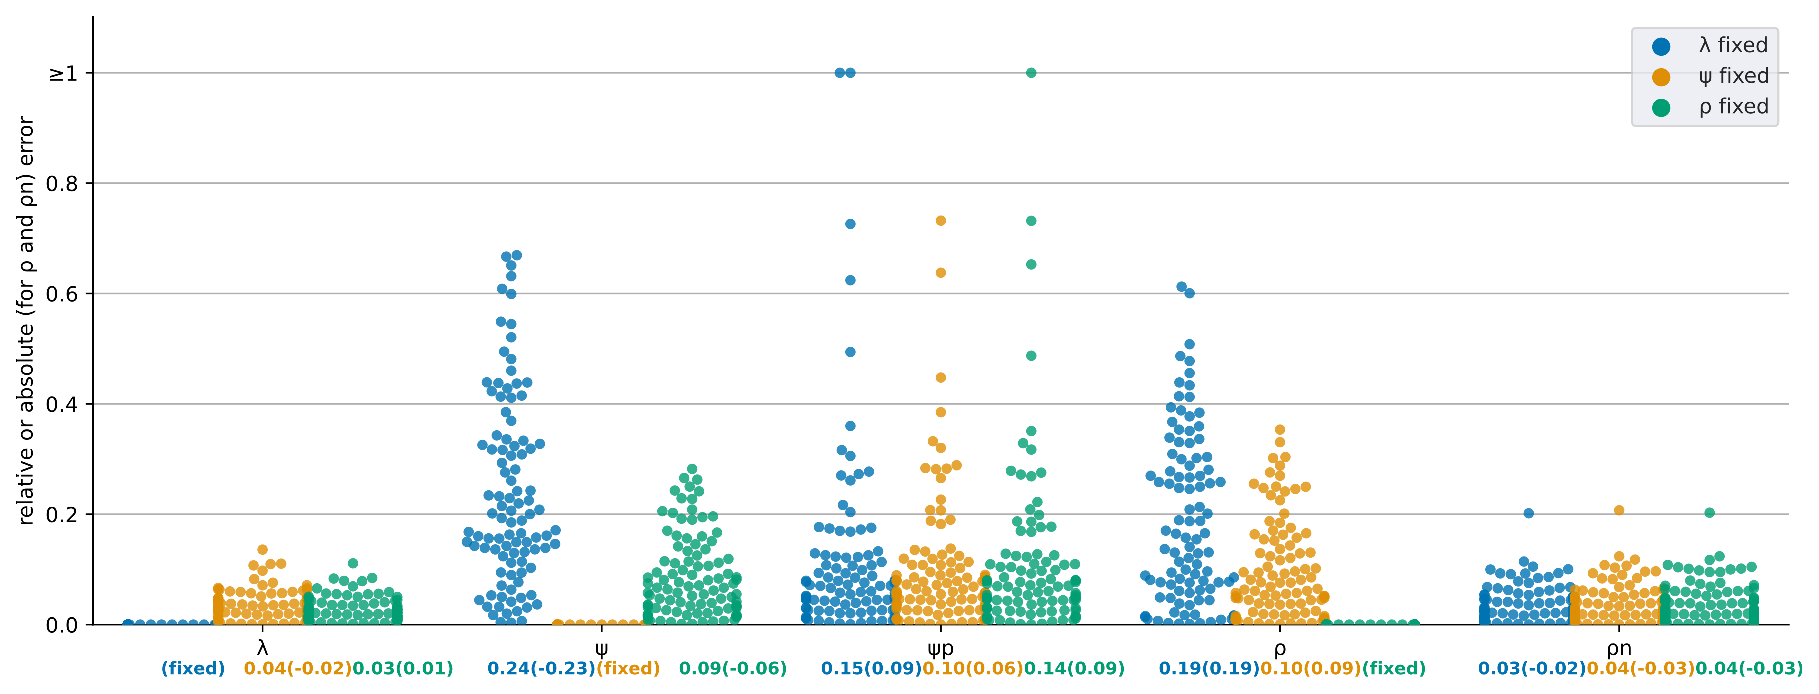
\includegraphics[width=1\textwidth]{Fig_errors.eps}
\caption{Comparison of inference accuracy of bdpn on a data set of 100 trees of 5\,000--10\,000 tips each, with either $\lambda$ (blue), $\psi$ (orange) or $\rho$ (green) parameter being fixed to its real value.
We show the swarmplots (coloured by fixed parameter) of relative errors for each test tree and parameter, which are measured as the normalized distance between the estimate and the real value. Average relative error (and in parentheses average bias, calculated on normalized values) are displayed for each parameter and method below their swarmplot. For $\rho$ absolute values are shown instead of normalized ones. } 
\label{fig:sim} 
\end{figure}
 
 \begin{table}[!h]\centering
\small
\caption{Percentage of simulated trees for which the real parameter values were withing the estimated 95\% CIs. \smallskip}
\begin{tabular}{c|ccc}
\textbf{parameter} & \textbf{$\lambda$ fixed} & \textbf{$\psi$ fixed} & \textbf{$\rho$ fixed} \\
\toprule 
 $\lambda$ & -- &  97\% & 96\% \\
 $\psi$ & 78\% & -- & 83\% \\
 $\rho$ & 28\% & 87\%  & -- \\
 $\psi_n$ & 94\% & 95\% & 95\% \\
 $\rho_n$ & 75\% & 76\% & 77\% \\
\bottomrule
\end{tabular}
\label{tbl:ci}
\end{table}

\subsection{Application: HIV-B epidemic in the UK}
We applied our estimator to asses the partner notification in HIV-infected patients in the UK. We used the dated phylogenetic tree from our recent study of HIV drug resistance in the UK~\citep{zhukovaModelingDrugResistance2023}. The tree represents the UK HIV-B epidemic between 1960s and 2017, its tips represent viruses sampled from 39\,159 individuals between 1996 and 2016. The samples come from the UK HIV Drug resistance database~\citep{Dunn2007}, which stores sequences from about 50\% of infected individuals in the UK~\citep{zhukovaModelingDrugResistance2023}. We therefore estimated the sampling probability $\rho$ as 0.5.

We cut this tree at year 2005, and estimated the BD-PN parameters on the 2005-on forests, in order to have a more homogeneous setting in terms of access to antiretroviral treatment, awareness of the HIV infection, etc. The 2005-on forest contained 18\,483 trees with a total of 31\,648 tips. We estimated the following parameter values: $\lambda=0.262$, $\psi=0.186$, $\psi_n=186.921$, $\rho_n=0.033$, which corresponds to $R_e = 1.4$, infectious time $\frac{1}{\psi} = 5.4$ years, and about 2 days between partner notification and their sampling.
 
The average time of HIV progression to AIDs in the absence of treatment is 10 years, which could serve as an estimate of the infectious time. However, in the UK, 95\% of infected population is on antiretroviral treatment, which, when taken properly, prevents transmission. Hence, the average infectious time represents the average time before starting treatment. Our estimate is approximately 5 years. 

To assess the robustness of these predictions with respect to $\rho$, we additionally estimated the parameter values for $\rho=0.4$ and for $\rho=0.6$. The results were very similar: $R_e$ of respectively $1.5$ and 
$1.3$, infectious time of $5.1$ and $5.6$ years, partner notification probability of $0.033$ in both cases and about 2 days between partner notification and their sampling.

\end{document}
